\documentclass[11pt]{beamer}

\usetheme{metropolis}


\usepackage[utf8]{inputenc}
\usepackage{ucs}
\usepackage[brazil]{babel}
\usepackage[T1]{fontenc}
\usepackage{amsmath}
\usepackage{amsfonts}
\usepackage{amssymb}
\usepackage{graphicx}
\usepackage{subfigure}
\usepackage{ragged2e}
\usepackage{fancybox}
\usepackage{tikz}



\usepackage{color}
\usepackage{fancyhdr}
\pagestyle{fancy}
\usepackage{xcolor}
\usepackage{xwatermark}

\title{CAPITULO 6 \\ Inferência de amostra pequena para uma proporção}
\author{Márcia}
\institute{Instituto de Matemática e Estatística \\Faculdade de Estatística}
\date{2019}

\begin{document}

\maketitle
%%%%%%%%%%%%%%%%%%%%%%%%%%%%%%%%%%%%

\section{Inferência de amostra pequena para uma proporção}

%%%%%%%%%%%%%%%%%%%%%%%%%%%%%%%%%%%%

\subsection{Paul o polvo}

%%%%%%%%%%%%%%%%%%%%%%%%%%%%%%%%%%%%

\begin{frame}
\frametitle{Preditores famosos}

\twocol{0.5}{0.5}{
Antes desse cara...
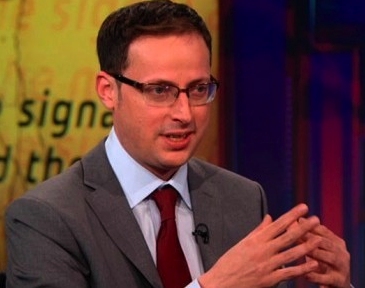
\includegraphics[width=\textwidth]{nate.png}
}
{
\pause
Tinha esse cara...
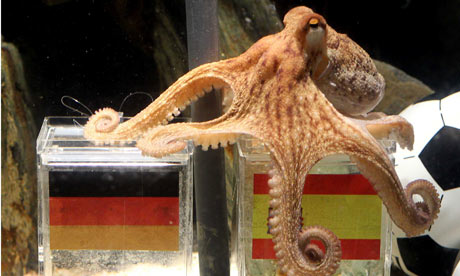
\includegraphics[width=\textwidth]{paul.png}
}

\end{frame}

%%%%%%%%%%%%%%%%%%%%%%%%%%%%%%%%%%

\begin{frame}
\frametitle{Paul o polvo - psíquico?}

\begin{itemize}

\item Paul o polvo previu 8 jogos da Copa do Mundo, e previu todos eles corretamente

\pause

\item Isso fornece evidências convincentes de que Paulo realmente tem poderes psíquicos?

\pause

\item Quão incomum seria se ele estivesse apenas adivinhando aleatoriamente (com 50 \% de chance de
adivinhando corretamente)?

\pause

\item Hipóteses:
\begin{itemize}
\item[$H_0:$] $p = 0.5$
\item[$H_A:$] $p > 0.5$
\end{itemize}

\end{itemize}

\end{frame}

%%%%%%%%%%%%%%%%%%%%%%%%%%%%%%%%%%

\begin{frame}
\frametitle{Condições}

\begin{enumerate}

\item \hl{Independência:} Podemos supor que cada palpite é independente de outro.

\pause

\item \hl{Tamanho da amostra:} O número de sucessos esperados é \orange {menor que 10}.
\[ 8 \times 0.5 = 4 \]

\end{enumerate}

\pause

\vspace{1cm}

\dq{Então, o que fazemos?}

\pause

Como o tamanho da amostra não é grande o suficiente para usar métodos baseados em CLT, usamos um método de simulação.

\end{frame}

%%%%%%%%%%%%%%%%%%%%%%%%%%%%%%%%%%

\begin{frame}
\frametitle{}

\pq{Qual dos seguintes métodos é a melhor maneira de calcular o valor p do teste de hipótese, avaliando se as previsões de Paul o polvo são excepcionalmente mais altas do que adivinhações aleatórias?}

\begin{enumerate}[(a)]
\item Jogue uma moeda 8 vezes, registre a proporção de vezes em que todos os 8 tiros foram de cara. Repita isso muitas vezes e calcule a proporção de simulações em que todos os 8 lançamentos foram cara.
\item Role um dado 8 vezes, registre a proporção de vezes em que todos os 8 rolos foram 6s. Repita isso várias vezes e calcule a proporção de simulações em que todos os 8 rolos foram 6s.
\item Jogue uma moeda 10.000 vezes, registre a proporção de cara. Repita isso várias vezes e calcule a proporção de simulações em que mais de 50 \% dos lançamentos são cara.
\item Jogue uma moeda 10.000 vezes, calcule a proporção de cara.
\end{enumerate}

\end{frame}

%%%%%%%%%%%%%%%%%%%%%%%%%%%%%%%%%%%

\begin{frame}
\frametitle{Simular}

\pq{Jogue uma moeda 8 vezes. Você conseguiu todas as caras?}

\begin{enumerate}[(a)]
\item Yes
\item No
\end{enumerate}

\end{frame}

%%%%%%%%%%%%%%%%%%%%%%%%%%%%%%%%%%

\begin{frame}[fragile]
\frametitle{}

{\tiny
\begin{Verbatim}[frame=single, formatcom=\color{blue}]
fonte ("http://www.openintro.org/stat/slides/inference.R")
paul = fator(c(rep("sim", 8), rep("não", 0)), nível = c("sim","não"))
inferência(paul, est = "proporção", tipo = "ht", método = "simulação",
          sucesso = "sim", nulo = 0.5, alternativo = "maior", semente = 290)
\end{Verbatim}
}

\pause

{\tiny
\begin{Verbatim}[frame=single, formatcom=\color{gray}]
Proporção única -- sucesso: sim
Estatísticas resumidas: p_hat = 1 ;  n = 8 
H0: p = 0.5 
HA: p > 0.5 
valor-p =  0.0037
\end{Verbatim}
}

\centering
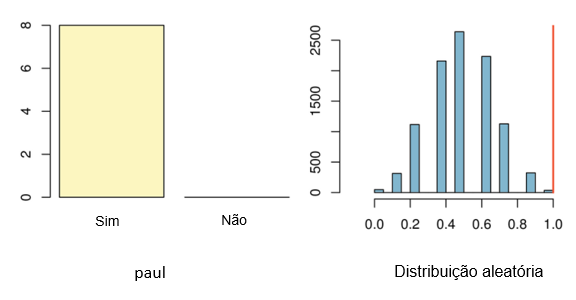
\includegraphics[width=0.8\textwidth,height=0.4\textheight]{paul_HT.pdf}

\end{frame}

%%%%%%%%%%%%%%%%%%%%%%%%%%%%%%%%%%%

\begin{frame}
\frametitle{Conclusões}

\pq{Qual das seguintes opções é \underline {falsa}??}

\begin{enumerate}[(a)]

\item Se, de fato, Paul estivesse adivinhando aleatoriamente, a probabilidade de ele obter o resultado de todos os 8 jogos corretos é 0,0037.

\item Rejeitar $ H_0 $, os dados fornecem evidências convincentes de que Paul fez melhor do que adivinhar aleatoriamente.

\item Podemos ter cometido um erro do Tipo I.

\solnMult{A probabilidade de que Paul seja psíquico é 0,0037.}

\end{enumerate}

\end{frame}

%%%%%%%%%%%%%%%%%%%%%%%%%%%%%%%%%%%%

\subsection{Back of the hand}

%%%%%%%%%%%%%%%%%%%%%%%%%%%%%%%%%%%

\begin{frame}
\frametitle{Dorso da mão}

\dq{Há um ditado que diz "conhece algo como a palma da sua mão". Descreva um experimento para testar se as pessoas realmente sabem as costas de suas mãos.}

\pause

\begin{center}
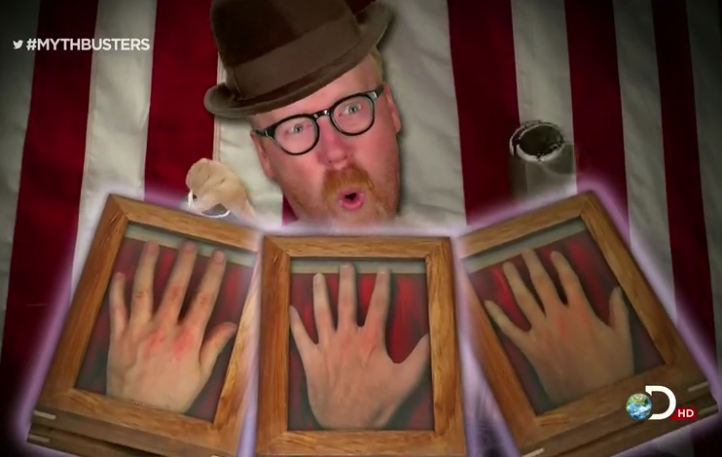
\includegraphics[width=0.6\textwidth]{mythbusters.png}
\end{center}

No episódio de MythBusters, 11 de 12 pessoas adivinham as costas de suas mãos corretamente.

\end{frame}

%%%%%%%%%%%%%%%%%%%%%%%%%%%%%%%%%%%%

\begin{frame}
\frametitle{Hipóteses}

\dq{Quais são as hipóteses para avaliar se as pessoas são capazes de reconhecer o dorso da mão a uma taxa melhor que a adivinhação aleatória. Lembre-se, no experimento MythBusters, havia 10 fotos para escolher, e apenas 1 estava correto.}

\begin{itemize}
\item[$H_0:$] $p = 0.10$ (adivinhação aleatória)
\item[$H_A:$] $p > 0.10$ (melhor do que adivinhar aleatoriamente)
\end{itemize}

\end{frame}

%%%%%%%%%%%%%%%%%%%%%%%%%%%%%%%%%%%

\begin{frame}
\frametitle{Condições}

\begin{enumerate}

\item \hl{Independência:} Podemos supor que cada pessoa que adivinhe é independente de outra.

\item \hl{Tamanho da amostra:} O número de sucessos esperados é \orange {menor que 10}.
\[ 12 \times 0.1 = 1.2 \]

\end{enumerate}

\dq{Então, o que fazemos?}

Como o tamanho da amostra não é grande o suficiente para usar métodos baseados em CLT, usamos um método de simulação.

\end{frame}

%%%%%%%%%%%%%%%%%%%%%%%%%%%%%%%%%%%

\subsection{Aleatorização HT para uma proporção}

%%%%%%%%%%%%%%%%%%%%%%%%%%%%%%%%%%%%

\begin{frame}
\frametitle{Esquema de simulação}

\dq{Descreva como você testa se os resultados desse experimento determinam se as pessoas são capazes de reconhecer o dorso da mão a uma taxa melhor do que a adivinhação aleatória.}
\vspace{-0.5cm}
\[ H_0: p = 0.10 \qquad H_A: p > 0.10 \qquad \hat{p} = 11 / 12 = 0.9167 \]

\begin{enumerate}

\item Use um dado justo de 10 lados para representar o espaço de amostragem, e chame 1 de sucesso (adivinhando corretamente), e todas as outras falhas de resultados (adivinhando incorretamente).


\item Jogue o dado 12 vezes (representando 12 pessoas no experimento), conte o número de 1s e calcule a proporção de palpites corretos em uma simulação de 12 rolos.

\item Repita o passo (2) muitas vezes, registrando a proporção de sucessos em uma série de 12 rolagens do dado.

\item Crie um gráfico de pontos das proporções simuladas a partir do passo (3) e conte o número de simulações em que a proporção foi pelo menos tão alta quanto 0,9167 (a proporção observada).

\end{enumerate}

\end{frame}

%%%%%%%%%%%%%%%%%%%%%%%%%%%%%%%%%%%

\begin{frame}
\frametitle{Resultados simulados}

\begin{itemize}

\item No próximo slide você pode ver os resultados de um teste de hipótese (usando apenas 100 simulações para manter as coisas simples).

\item Cada ponto representa uma proporção de sucesso da simulação. Houve 25-30 simulações em que a taxa de sucesso ($ \hat {p} $) foi de 10 \%, 40-45 simulações em que a taxa de sucesso foi ligeiramente inferior a 10 \%, cerca de 20 simulações em que a taxa de sucesso foi ligeiramente menor de 20 \% e 1 simulação em que a taxa de sucesso foi superior a 30 \%.

\item Não há simulações em que a taxa de sucesso seja tão alta quanto a taxa de sucesso observada de 91,67 \%.

\item Portanto, concluímos que o resultado observado é quase impossível de acontecer por acaso (p-valor = 0).

\item E, portanto, esses dados sugerem que as pessoas são capazes de reconhecer as costas de suas mãos a uma taxa melhor do que adivinhar aleatoriamente.

\end{itemize}

\end{frame}

%%%%%%%%%%%%%%%%%%%%%%%%%%%%%%%%%%%%

\begin{frame}[fragile]
\frametitle{}

{\tiny
\begin{Verbatim}[frame=single, formatcom=\color{blue}]
costas = as.factor(c(rep("correto", 11), rep("errado", 1))) 
inferência(costas, est = "proporção", tipo = "ht", método = "simulação",
	sucesso = "correto", nulo = 0.1, alternativo = "maior", semente = 654, nsim = 100)
\end{Verbatim}
}

\pause

{\tiny
\begin{Verbatim}[frame=single, formatcom=\color{gray}]
Proporção única - sucesso: correto 
Estatísticas resumidas: p_hat = 0.9167 ;  n = 12 
H0: p = 0.1 
HA: p > 0.1 
p-value =  0 
\end{Verbatim}
}

\centering
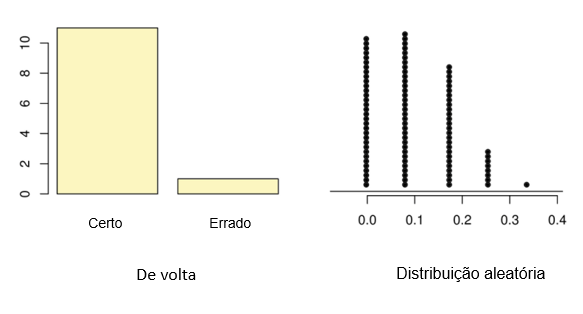
\includegraphics[width=0.8\textwidth,height=0.4\textheight]{back_HT.pdf}

\end{frame}

%%%%%%%%%%%%%%%%%%%%%%%%%%%%%%%%%%%

\end{document}
